%% This work is distributed under the LaTeX Project Public License (LPPL)
%% ( http://www.latex-project.org/ ) version 1.3, and may be freely used,
%% distributed and modified. A copy of the LPPL, version 1.3, is included
%% in the base LaTeX documentation of all distributions of LaTeX released
%% 2003/12/01 or later.
%% Retain all contribution notices and credits.
%% ** Modified files should be clearly indicated as such, including  **
%% ** renaming them and changing author support contact information. **
%%*************************************************************************
\documentclass[conference]{IEEEtran}
\usepackage{fontspec}
\setmainfont[
 Path = ./ ,
 Extension = .otf ,
 Mapping=tex-text,
 Ligatures={TeX, Common},
 BoldFont = texgyretermes-bold,
 ItalicFont = texgyretermes-italic,
 BoldItalicFont = texgyretermes-bolditalic,
 SmallCapsFont = texgyretermes,
 SmallCapsFeatures = {Letters = SmallCaps}
]{texgyretermes}

\usepackage{polyglossia}
\setdefaultlanguage{russian}
\setotherlanguages{english}

\usepackage[backend=biber,style=ieee,refsection=section]{biblatex}    
% *** CITATION PACKAGES ***
%
% \usepackage{cite}
% cite.sty was written by Donald Arseneau
% V1.6 and later of IEEEtran pre-defines the format of the cite.sty package
% \cite{} output to follow that of the IEEE. Loading the cite package will
% result in citation numbers being automatically sorted and properly
% "compressed/ranged". e.g., [1], [9], [2], [7], [5], [6] without using
% cite.sty will become [1], [2], [5]--[7], [9] using cite.sty. cite.sty's
% \cite will automatically add leading space, if needed. Use cite.sty's
% noadjust option (cite.sty V3.8 and later) if you want to turn this off
% such as if a citation ever needs to be enclosed in parenthesis.
% cite.sty is already installed on most LaTeX systems. Be sure and use
% version 5.0 (2009-03-20) and later if using hyperref.sty.
% The latest version can be obtained at:
% http://www.ctan.org/pkg/cite
% The documentation is contained in the cite.sty file itself.

\usepackage{graphicx}
\usepackage{amsmath}
\usepackage{url}
\usepackage{array}
\usepackage[caption=false,font=footnotesize]{subfig}
\usepackage{lipsum}
% \usepackage[caption=false,font=footnotesize]{subfig}
% \usepackage{dblfloatfix}
% The latest version can be found at:
% http://www.ctan.org/pkg/dblfloatfix

\renewcommand{\thesubsection}{\Alph{subsection}.}
\renewcommand{\thesubsubsection}{\arabic{subsubsection})}
\renewcommand{\theparagraph}{\alph{paragraph})}


% The following code makes "fake small caps" which work fine
% for cyrillic symbols
% Borrowed from http://tex.stackexchange.com/questions/64582/faking-small-caps-in-xelatex?rq=1


\usepackage{expl3,xparse}

% turn expl3 space on: `:' and `_' are letters now and spaces
% are ignored. To insert a space use `~'.
\ExplSyntaxOn
% the internal command:
\cs_new:Npn \fakecaps:n #1
  {
    \addfontfeature{LetterSpace=10.0} {\tl_head:n { #1 }\kern 1pt}{\addfontfeature{Scale=0.9}\uppercase{\tl_tail:n { #1 }}}
  }

% the document command:
\NewDocumentCommand\FakeCaps{m}
  {\fakecaps:n { #1 } }

% turn expl3 space off again:
\ExplSyntaxOff

\makeatletter
\newcommand\subparagraph{%
  \@startsection{subparagraph}{5}
  {\parindent}
  {3.25ex \@plus 1ex \@minus .2ex}
  {-1em}
  {\normalfont\normalsize\bfseries}}
\makeatother
\usepackage[explicit]{titlesec}
\let\subparagraph\relax
\titleformat{\section}[hang]{\normalfont\normalsize\centering}{\thesection.}{0.5em}{\FakeCaps{#1}}

\makeatletter
\def\russian@capsformat{}
\makeatother

\usepackage{listings}
\usepackage{hyperref}
\usepackage{verbments}
\usepackage{minted}
\usepackage{caption}
\usepackage{fancybox}
%% \usepackage{cite}
\newfontfamily{\cyrillicfonttt}{DejaVu Serif}

\makeatletter
\define@key{blx@lbx}{fromjapanese}{\blx@defstring{fromjapanese}{#1}}
\define@key{blx@lbx}{langjapanese}{\blx@defstring{langjapanese}{#1}}
\makeatother

\lstset{
basicstyle=\small,
identifierstyle=\ttfamily,
keywordstyle=\bfseries,
commentstyle=\scriptsize\rmfamily,
basewidth={0.5em,0.5em},
fontadjust=true,
escapechar=~,
language=java
}

%% Bibliography file
%% \addbibresource{seim.bib}


% If you need to correct hyphenations, add them here
\hyphenation{op-tical net-works semi-conduc-tor}

\newcommand{\igo}[1]{{\color{red}({Игорь:\ #1})}\marginpar{!}}
\newcommand{\app}[1]{{\color{blue}({Антон:\ #1})}\marginpar{!}}

\begin{document}
%
% paper title
%
% In English titles are generally capitalized except for words such as a, an, and, as,
% at, but, by, for, in, nor, of, on, or, the, to and up, which are usually
% not capitalized unless they are the first or last word of the title.
% Linebreaks \\ can be used within to get better formatting as desired.
% Do not put math or special symbols in the title.
\title{Генерация декларативных форматеров по грамматике в форме Бэкуса-Наура}


% author names and affiliations
% use a multiple column layout for up to three different
% affiliations
\author{\IEEEauthorblockN{Игорь Озерных}
\IEEEauthorblockA{Санкт-Петербургский\\Государственный Университет\\
st011628@student.spbu.ru}
\and
\IEEEauthorblockN{Антон Подкопаев}
\IEEEauthorblockA{Санкт-Петербургский\\Государственный Университет\\
a.podkopaev@2009.spbu.ru}
}

% make the title area
\maketitle

% As a general rule, do not put math, special symbols or citations
% in the abstract
\begin{abstract}
Одним из декларативных подходов к заданию средств форматирования кода (СФК)
является метод \emph{синтаксических шаблонов}, которые
являются примерами представления (форматирования) синтаксических
конструкций целевого языка.
Для извлечения шаблонов из предоставленного \emph{образца},
кодовой базы на целевом языке с желаемым стилем форматирования,
используется (не кооперативный) синтаксический анализатор. 

Недостатком существующей системы является то, что 
%% форматирования с использованием синтаксических шаблонов
для получения форматера нового целевого языка
необходимо вручную реализовать языкозависимую прослойку между ядром
системы и представлением синтаксического
дерева, получаемого в результате работы анализатора.
Этот процесс трудоёмок и требует глубоких знаний о системе.

%% Упомянутая прослойка достаточно велика и сложна, поскольку представление
%% дерева имеет размер (количество соответствующих ему классов),
%% пропорциональный числу конструкций целевого языка.
%% Кроме того, существующая система предполагает создание данной прослойки
%% вручную.

Данная работа посвящена автоматическому получению такой прослойки
для случая, когда синтаксический анализатор генерируется из грамматики языка в
расширенной форме Бэкуса-Наура.
Реализация выполнена в виде расширения плагина Grammar-Kit
для среды разработки IntelliJ IDEA, позволяющего
по грамматике в форме Бэкуса-Наура получить и синтаксический анализатор,
и декларативное СФК для целевого языка.
В рамках апробации разработанная система была использована
для получения СФК по грамматикам учебного языка While
и языка Erlang.
\app{TODO: Проверить, что всё хорошо с Erlang.}
\end{abstract}

\section{Введение}
%% Автоматическое форматирование текстов программ является
%% классической задачей, возникающей в контексте различных 
%% языковых процессоров, например, сред разработки (IDE) и декомпиляторов.

%% Одним из подходов к решению данной задачи является
%% \emph{декларативное форматирование}. Оно позволяет
%% определить форматер по множеству \emph{синтаксических шаблонов}, т.е.
%% примеров представления (форматирования) синтаксических конструкций.
%% Шаблоны, в свою очередь, могут быть извлечены
%% из некоторого образца --- кодовой базы с желаемым стилем форматирования
%% на целевом языке.

%% Для извлечения шаблонов используется кооперативный синтаксический анализатор
%% целевого языка.


%% Недостатком декларативных форматеров является относительная сложность их
%% реализации для новых целевых языков --- необходимо иметь кооперативный
%% синтаксический анализатор целевого языка.

%% Существуют реализации декларативных форматеров для Java и учебного
%% языка While.
%% Недостатком существующих декларативных форматеров является 

На этапе поддержки и сопровождения в жизненном цикле ПО особенно важным является понимание программного текста поддерживаемой системы. 
% * <podkoav239@gmail.com> 23:37:26 15 Apr 2016 UTC+0300:
% Предыдущие 2 предложения не нужны.
Для этого необходимо сделать код легко читаемым, то есть форматировать его.
Форматирование каких элементов необходимо произвести и каким образом определяется стандартом кодирования (CK, coding convention).
Например, для языка программирования C++ наиболее популярными являются следующие стандарты кодирования: Google\footnote{\texttt{https://google-styleguide.googlecode.com/svn/trunk/cppguide.html}}, GNU\footnote{\texttt{http://www.gnu.org/prep/standards/standards.html}}, BSD\footnote{\texttt{https://www.freebsd.org/cgi/man.cgi?query=style\&sektion=9}}.

Существуют различные подходы к форматированию кода. Одним из них является использование форматеров (программ, форматирующих код).
Современные интегрированные среды разработки (IDE), такие как IntelliJ IDEA, Visual Studio, Eclipse и др.,~--- включают в себя форматеры.
Желаемый стиль кодирования задается с помощью множества настроек. Например, расположение открывающей фигурной скобки (на той же строке или на новой), количество пробелов в отступе (для операторов внутри фигурных скобок) и т.д.

Недостатком этого подхода является необходимость вручную задавать настройки форматирования, что может быть неудобным при переходе от одного СК к другому.
Кроме того, количество принципиально разных стилей форматирования, которых можно задать с помощью данных настроек, невелико.
Например, настройки форматеров приведенных IDE не позволяют задавать форматирование, подобное S-выражениям языка Lisp.
%выразить СК, в котором закрывающая фигурная скобка ставится на той же строке, что и последний оператор блока (см. рис.~\ref{fig:unusualCC}).
\begin{figure}[h]
	\centering
	\lstinputlisting[language=c]{codes/unusualCC.txt}
	\caption{Нестандартный СК}
	\label{fig:unusualCC}
\end{figure}

Альтернативный подход к форматированию описан в статье~\cite{while} и основывается на сопоставлении с образцом и синтаксических шаблонах.
Под \emph{шаблоном} понимаются данные, сопоставление которых с элементом синтаксического дерева дает текстовое представление этого элемента.

Например, на рис.~\ref{fig:ifTree} представлено дерево разбора для оператора ветвления. 
\begin{figure}[h]
	\centering
	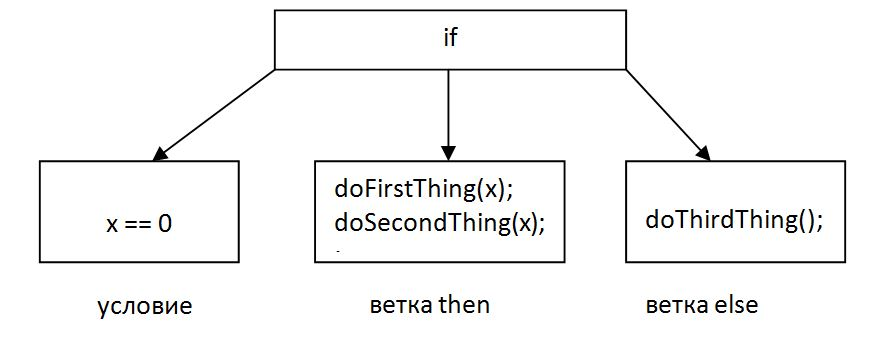
\includegraphics[width=.5\textwidth]{images/ifTree.jpg}
	\caption{Представление оператора ветвления в виде дерева разбора}
	\label{fig:ifTree}
\end{figure}

На рис.~\ref{fig:tmpltcodeintro}а изображен шаблон форматирования, который может быть применен к нему (несколько подвыражений, соответствующих выполнению условия, и одно подвыражение, соответствующее невыполненению условия).
На рис.~\ref{fig:tmpltcodeintro}б представлен результат применения этого шаблона к дереву разбора для оператора ветвления.

\fvset{frame=lines,framesep=6pt}
\begin{figure}[ht]
\noindent\begin{minipage}{.2\textwidth}
    \lstinputlisting[language=Java]{codes/ifTemplateIntro.txt}
\caption*{а) Шаблон для оператора ветвления}    
\end{minipage}\hfill
\begin{minipage}{.25\textwidth}
    \lstinputlisting[language=Java]{codes/ifCodeIntro.txt}
\caption*{б) Текст, полученный при применении шаблона к дереву разбора}    
\end{minipage}
\caption{Оператор ветвления и шаблон для него}    
\label{fig:tmpltcodeintro}
\end{figure}

Отличием этого подхода от классических форматеров является то, что вместо настроек используется репозиторий, содержащий код с желаемым форматированием.
Подобные форматеры мы будем называть \emph{декларативными}.
Декларативность достигается путем вычленения из образца синтаксических шаблонов для конструкций целевого языка и построения с их помощью представлений для переданных на форматирование программ.

В статье был рассмотрен метод создания форматеров для различных языков программирования, которые настраиваются на требуемый СК по образцу кода, а в качестве апробации разработаны декларативные форматеры для языков Java, Haskell~\cite{korDiploma} и учебного языка While.
Выбор языка Java обусловлен тем, что Си-подобный синтаксис очень распространен, а значит, метод, применимый для Java, можно распространить и на множество других языков.
В Haskell форматирование является неотъемлемой частью языка и влияет на его синтаксическую корректность. 
Применимость метода к таким разным языкам показывает, что он может быть также применен на множестве других языков программирования.

Эти форматеры генерировались по специальному XML-описанию конструкций языка (одна конструкция~--- один файл с описанием). 
В это описание входят название структуры языка, класс синтаксического анализатора в платформе IntelliJ IDEA, список поддеревьев (листинг~\ref{fig:whileXml}).

\begin{figure}[h]
	\centering
	\lstinputlisting[language=c]{codes/whileXml.txt}
	\caption{XML-описание структуры ``if'' языка While}
	\label{fig:whileXml}
\end{figure}

Недостатком такого подхода является то, что в языке может быть большое количество конструкций (While~--- около двадцати, Erlang~--- более ста).
В связи с этим, создание такого описания компонент языка может быть весьма трудоемким.

В статье~\cite{while} указывается на то, что для языков, не имеющих поддержки со стороны IntelliJ IDEA, необходимо сначала получить синтаксический и лексический анализаторы.
Сделать это можно с помощью плагина Grammar-Kit\footnote{\texttt{https://github.com/JetBrains/Grammar-Kit}} путем их генерации по грамматике в форме Бэкуса-Наура.
Для уменьшения трудозатрат по созданию декларативного форматера можно использовать те же входные данные, что используются для генерации анализаторов, то есть грамматику языка.

Целью данной работы является описание метода генерации декларативных принтеров по грамматике языка в форме Бэкуса-Наура, интеграции этого метода в плагин Grammar-Kit и апробации этого метода на примере учебного языка While.


\section{Обзор}
Существует достаточно много различных подходов к форматированию
программного кода.
Наиболее близкий к нашей работе метод описан в \cite{Brand-Visser:ACM96}.
В этой работе форматер может быть получен по ASF+SDF \cite{Klint:ACM93}
описанию языка, которое представляет собой проаннотированную грамматику.
Сначала по грамматике строится тривиальный форматер (unparser) путём
рассмотрения продукций грамматики как правил форматирования,
где между всеми токенами вставляется по одному пробельному символу.
Далее, на основе тривиального форматера генерируется настоящий
форматер с помощью применения нескольких эвристик,
почерпнутых из стандартов форматирования Algol-подобных языков.
%% Причём для полученного форматера тривиальным образом верно, что он
%% порождает программный текст, который соответствует грамматике языка.
Разработчик, использующий описываемую систему, также может вручную поменять
часть правил форматирования.
Недостатком является то, что правила форматирования ``зашиты'' в
описание грамматики, и могут быть модифицированы только разработчиком,
в отличие от нашего подхода, позволяющего пользователю декларативным
образом настраивать форматер.
%% , но с потерей последнего свойства.

Одними из наиболее часто встречающихся на практике форматеров можно считать
форматеры, встроенные в среды разработки --- IntelliJ IDEA, Eclipse,
Visual Studio и т.д.
\app{TODO: написать про IDEA/Eclipse и навороты с Machine Learning.}


\section{Генерация декларативных форматеров}
Для генерации декларативных принтеров будет использоваться БНФ-грамматика, по которой генерируются синтаксический и лексический анализатор соответствующими генераторами в плагине Grammar-Kit.
Наша цель изменить грамматику таким образом, чтобы из нее можно было извлечь все необходимые данные для генерации декларативных форматеров.
\subsection{Изменения в грамматике}
Помимо описания синтаксиса языка, грамматика содержит некоторые дополнительные данные, необходимые генератору синтаксического анализатора.
Среди этих данных, например, будущие зависимости классов, Java-пакеты, префиксы и суффикcы сгенерированных классов и др.

\subsubsection*{Генерация компонент форматера для списковых структур}
\emph{Компонентой} форматера является класс, описывающий, каким образом должна форматироваться данная структура языка.
В работе~\cite{while} описываются особенности форматирования списковых структур языка.
Поэтому заранее необходимо знать, является ли структура списком, чтобы сгенерировать для нее корректную компоненту.
В связи с этим появилась необходимость в дополнительном обозначении таких структур.
Если правило описывает некоторую списочную конструкцию, то дополнительно указывается модификатор \emph{list}.
Это позволяет явно указать шаблон для их генерации.

\subsubsection*{Генерация файловой компоненты}
Каждая сгенерированная компонента форматера использует соответствующий Psi-класс (``\emph{Psi}''~--- стандартный префикс классов синтаксических узлов в платформе IntelliJ IDEA).
Файловая компонента не является исключением, однако генератор синтаксического анализатора не генерирует соответствующий Psi-узел, и поэтому он всегда создается вручную.
Способ создания такого класса не подчиняется строгим правилам и может иметь вариации, поэтому возникает множество трудностей при генерации (разное количество поддеревьев, которое можно получить с помощью генератора и которое предоставляется Psi-узлом; несоответствие имен методов и др.).
Решением этой проблемы стало явное задание поддеревьев, которые будут сгенерированы.
Например, поддеревья языка Java можно задать следующим образом: \lstinline[language=java]{fileSubtrees="PackageStatement, ImportList, Classes*"}.
Названия поддеревьев соответствуют методам Psi-узла, ``*'' указывает, что поддерево является массивом или списком.


\subsection{Выделение значимых элементов}
Первое, что необходимо сделать~--- выделить значимые элементы языка. 
Под \emph{значимыми} понимаются элементы, которым потенциально нужно будет менять форматирование.
Помимо описанного выше модификатора для списков, у правил есть и другие модификаторы.
Среди них: private, external~--- для таких правил не генерируются компоненты форматера исходя из тех соображений, что и генератор синтаксического анализатора не создает для них Psi-узлов .
Правило с отличными от указанных выше модификаторами считается значимым при выполнении следующих условий: оно не является цепным или леворекурсивным.

\subsection{Определение поддеревьев}
После того, как определены все значимые структуры языка, необходимо понять, из каких подструктур они состоят.
Используя XML-описания, мы могли явно указывать поддеревья для какой-либо компоненты.
Теперь же всю информацию о поддеревьях можно получить прямо из правила грамматики.
\emph{Поддеревом} в контексте данной работы будет являться терминал или значимый нетерминал в правой части правила.

\subsection{Генерация}
После определения значимых правил и их поддеревьев происходит генерация кода компонент языка.

Так как компоненты принципиально мало отличаются друг от друга, то для генерации можно использовать файлы-шаблоны, в которых существует множество меток вида \lstinline[language=java]{@TEXT@} для вставки соответствующей информации.
На рис.~\ref{component} изображен шаблон для генерации компоненты форматера.
\begin{figure}[h]
	\centering
	\lstinputlisting[language=java]{codes/component.txt}
	\caption{Шаблон для генерации компонент}
	\label{component}
\end{figure}

\section{Апробация}
На рис.~\ref{whileBnf} изображена часть итоговой грамматики языка While.
Она подается на вход генератору принтера, который автоматически сгенерирует форматер и его компоненты.
По этой грамматике генерируется 19 компонент (в общем, 2200 строк кода).
Этого количества достаточно для форматирования программ, написанных на этой языке.

\begin{figure}[h]
	\centering
	\lstinputlisting[language=xml]{codes/whileBnf.txt}
	\caption{Часть БНФ-грамматики языка While}
	\label{whileBnf}
\end{figure}

\subsection{Пример работы декларативного форматера для языка While}
Рассмотрим программу на языке While (см. листинг~\ref{whileProg}).
На листингах~\ref{whileTs} а и б приведены программы, которые будут использованы для форматирования листинга~\ref{whileProg}.
Результаты форматирования приведены на листинге~\ref{whileRes}.
Полученный код является синтаксически корректным и имеет то же форматирование, что переданный на вход шаблон.

\begin{figure}[h]
	\centering
	\lstinputlisting[language=xml]{codes/whileProg.txt}
	\caption{Пример программы на языке While}
	\label{whileProg}
\end{figure}

\fvset{frame=lines,framesep=6pt}
\begin{figure}[ht]
\noindent\begin{minipage}{.2\textwidth}
    \lstinputlisting[language=Java]{codes/whileT1.txt}
\caption*{а)}    
\end{minipage}\hfill
\begin{minipage}{.2\textwidth}
    \lstinputlisting[language=Java]{codes/whileT2.txt}
\caption*{б)}    
\end{minipage}
\caption{Образцы форматирования}    
\label{whileTs}
\end{figure}

\fvset{frame=lines,framesep=6pt}
\begin{figure}[ht]
\noindent\begin{minipage}{.2\textwidth}
    \lstinputlisting[language=Java]{codes/whileRes1.txt}
\caption*{а)}    
\end{minipage}\hfill
\begin{minipage}{.2\textwidth}
    \lstinputlisting[language=Java]{codes/whileRes2.txt}
\caption*{б)}    
\end{minipage}
\caption{Результат форматирования программы из листинга~\ref{whileProg}}
\label{whileRes}
\end{figure}

\section{Заключение}
В рамках исследования была разработана методика генерации декларативных форматеров по грамматике в форме Бэкуса-Наура.
Соответствующая функциональность реализована в рамках проекта Grammar-Kit.
Корректность работы была проверена на примере генерации форматера учебного языка While.

Ограничением данного подхода является необходимость наличия грамматики языка в форме, понятной плагину Grammar-Kit. 
Если же грамматика уже существует, то необходимо вручную найти в ней правила для списочных структур и отметить их модификатором \emph{list}.
Кроме того, платформа для поддержки новых языков в IntelliJ IDEA подразумевает наличие фабрики элементов, преобразующей программный текст структур языка в объекты, которыми оперирует система.
Если форматер разрабатывается для языка, поддержки которого ранее не было, то фабрику элементов можно сгенерировать или написать вручную понятным для форматера образом.
В случае, если форматер генерируется для языка, для которого уже есть поддержка в системе (а значит, есть и фабрика элементов), то необходимо создать посредника между ними для обеспечения взаимодействия.

Кроме того, данная реализация применима лишь для платформы IntelliJ IDEA, однако идею можно распространить и на другие платформы.

% use section* for acknowledgment
\section*{Благодарности}
Работа выполнена при поддержке компании JetBrains\footnote{https://jetbrains.com}.

% references section
\nocite{*}

%% \printbibliography
%% \bibliographystyle{abbrv}
%% \bibliography{seim}

\begin{thebibliography}{4}

\bibitem{korDiploma}
  А. Коровянский. Абстрактная печать по образцу
  // Дипломная работа, МатМех СПбГУ, 2015.

\bibitem{while}
  А. Подкопаев, А. Коровянский, И. Озерных.
  Языконезависимое форматирование текстов программ
  на основе сопоставления с образцом и синтаксических шаблонов
  // НТВ СПбГПУ 4' (224), 2015.

\bibitem{podkopaevDiploma}
  А. Подкопаев. Полиномиальной сложности оптимальные принтер-комбинаторы с выбором
  // Дипломная работа, МатМех СПбГУ, 2014.
  
\bibitem{maintenance}
  G. Alkhatib.
  The maintenance problem of application software:
an empirical analysis //
  Journal of Software Maintenance, 4(2):83–104, 1992.
  
\bibitem{Brand-Visser:ACM96} M. van den Brand and E. Visser.
Generation of formatters for context-free languages //
ACM Trans. Softw. Eng. Meth. 5, 1, p1-41, 1996.

\bibitem{Klint:ACM93} P. Klint. A Meta-environment for Generating Programming Environments //
ACM Trans. Softw. Eng. Meth. 2, 2, p176-201, 1993.


\bibitem{Corbo-al:ICSM07} F. Corbo, C. Del Grosso, M.Di Penta.
Smart Formatter: Learning Coding Style from Existing Source Code //
ICSM. 2007.

\end{thebibliography}

\end{document}

